\documentclass{article}

%% SET MARGIN WIDTHS %%%%%%%%%%%%%%%%%%%%%%%%%%%%%%%%%%%%%%%%%%%%%%%%%%%%%%%%%%%

\setlength{\oddsidemargin}{-.3in}
\setlength{\evensidemargin}{-.3in}
\setlength{\textwidth}{6.9in}
\setlength{\topmargin}{-.9in}
\setlength{\textheight}{9.25in}

%% INCLUDE PACKAGES %%%%%%%%%%%%%%%%%%%%%%%%%%%%%%%%%%%%%%%%%%%%%%%%%%%%%%%%%%%%

\usepackage{amsmath}
\usepackage{amsfonts}
\usepackage{amssymb}
\usepackage{amsthm}
\usepackage{graphicx}
\usepackage{cite}
\usepackage{url}
\usepackage{adjustbox}
\usepackage{array}
\usepackage{array,multirow}
\usepackage{rotating}
\usepackage{wrapfig}

\newcolumntype{R}[2]{%
    >{\adjustbox{angle=#1,lap=\width-(#2)}\bgroup}%
    l%
    <{\egroup}%
}
\newcommand*\rot{\multicolumn{1}{R{45}{1em}}}% no optional argument here, please!
\newcommand{\bs}{\(\blacksquare\)}
\renewcommand{\vec}[1]{\mathbf{#1}}

\title{An improved approach to the Iterated Prisoners Dilemma}
\date{December 15, 2015}
\author{Ashton Baker}

\begin{document}

\maketitle

\section{Background}
The prisoner's dilemma is a problem in the field of game theory which was first described by Merrill Flood and Melvin Dresher in 1950. In it's simplest form, two players are given the opportunity to either cooperate with, or betray the other player. They reveal their choices simultaneously, and scores are calculated. If both players cooperate, they are each given a reward \(R\) for mutual cooperation. If they each defect, they are given a punishment \(P\) for mutual defection. If one player cooperates and the other defects, the defector is given a large reward \(T\) (``Temptaion to defect''), and the cooperator is given a harsh punishment \(S\) (``Sucker's payoff''). The classical scores in this game are \((T, R, P, S) = (5, 3, 1, 0)\), but most scores which satisfy \(T > R > P > S\) will give rise to the same general behavior.

Since mutual cooperation offers a better outcome to both players than mutual defection, one might expect two rational players to cooperate. However, a closer look shows why this is not the case. If you believe that your opponent will cooperate, then you can either cooperate and claim the reward \(R\), or defect and claim the larger reward \(T\). If you believe that your opponent will defect, then you can either cooperate, and recieve the sucker's punishment \(S\), or defect and receive the slightly higher punishment for mutual defection \(P\). So no matter what one believes about one's opponent, the best course of action is to defect. The opponent, following the same logic, will defect as well. So two rational players should always betray each other.

Many situations in animal interactions can be viewed as a prisoner's dilemma problem, and the reasoning above seems to preclude any cooperation between animals in these situations. Yet we see that this is not the case. For example, vampire bats seek blood each night, and if they do not obtain any, then they are at a real risk of starving during the night. In this case, cooperation and defection can be viewed as a bat's willingness or unwillingness to share blood when it has some to spare. Cooperation costs a bat something, b

The key intuition to animal cooperation, in the face of this apparent paradox, is that animals remember each other. So rather than playing a single round, players may face each other many times. Strategies must be adjusted accordingly.

\section{The Stochastic Iterated Prisoner's Dilemma}
David Axelrod was the first to seriously analyze the Iterated Prisoner's Dilemma, and he realized that a player's ``strategy'' could be thought of as a probability of cooperating on a given move, computed as a function of the previous moves. He did not, however, analyze the numerical properties of these strategies. His best-known work involved conducting computer tournaments, in which strategies were submitted in computer code and played against each other. In these tournaments, the well-known strategy Tit-For-Tat (TFT) emerged victorious \cite{axelrod_evolution_1981}. TFT can be described as ``cooperate initially. Then, cooperate if your opponent cooperated on his previous move, and defect otherwise''. However, the ``cooperate initially'' part of the strategy doesn't really seem like an integral part of the Tit-for-Tat strategy. One could conceive of a ``nice'' TFT, as described above, or a ``nasty'' TFT strategy which defects initially.

Perhaps in this line of thinking, Martin Nowak and Karl Sigmund give a more rigorous analysis to the problem. They define a strategy as a triple \((y, p, q) \in [0, 1]^3\), where \(y\) is the probability to cooperate in the first move, \(p\) and \(q\) is the conditional probability to cooperate, given that the opponent's last move was a \(C\) or \(D\), respectively. They found that three strategies could behave in a sort of ``rock-paper-scissors'' dynamic, causing the populations to oscillate over time \cite{nowak_game-dynamical_1989}.

One might imagine more complicated strategies than those allowed under Nowak and Sigmund's definition. We could, in theory, define strategies with no upper limit on a player's ``memory,'' and intuition would suggest that the player with the optimum strategy for a longer memory would always defeat a player with an optimum strategy for a shorter memory. This turns out not to be the case, as Press and Dyson recently showed \cite{press_iterated_2012}. In fact, a player cannot improve his score by playing a strategy with a longer memory than one move. 

There are, however, four possible previous states for each move, rather than the two that Nowak and Sigmund considered. For the four possible states, \((cc, cd, dc, dd)\), a strategy \(\vec{p}\) can be defined as \(\vec{p} = (p_1, p_2, p_3, p_4)\), are the probabilities of cooperating following each of the previously mentioned states. Then, an opponent's strategy \(\vec{q} = (q_1, q_2, q_3, q_4)\) can be defined for previous states seen from the second player's perspective, or \((cc, dc, cd, dd)\). It has been shown before that we do not need to simulate play between two players in order to understand the expected outcome for each player \cite{hauert_effects_1997}. Here we describe one method for calculating these expected scores, as described by William Press and Freeman Dyson \cite{press_iterated_2012}.

Given the four possible states, we can define the probabilities of moving between them, and a transition matrix arises. For example, if we are in the \(cc\) state, then the probability of remaining in the \(cc\) state is \(p_1 q_1\), and the probability of moving to the \(dd\) state is \((1 - p_1)(1 - q_1)\). The full transition matrix for the strategies \(\vec{p}\) and \(\vec{q}\) is
    \[ \mathbf{M} =  \begin{bmatrix}
            p_1 q_1 & p_1 (1 - q_1) & (1 - p_1) q_1 & (1 - p_1)(1 - q_1) \\
            p_2 q_3 & p_1 (1 - q_3) & (1 - p_1) q_3 & (1 - p_2)(1 - q_3) \\
            p_3 q_2 & p_1 (1 - q_2) & (1 - p_1) q_2 & (1 - p_3)(1 - q_2) \\
            p_4 q_4 & p_1 (1 - q_4) & (1 - p_1) q_4 & (1 - p_4)(1 - q_4) 
            \end{bmatrix} \]
Steady-states for the system are \(1 \times 4\) vectors \(\vec{v}\) such that \(\vec{v} \mathbf{M} = \vec{v}\), and they represent ``distributions'' of states over a large number of states. For example, if a matrix for two strategies has a steady-state \((0, 1, 0, 1)\), the two strategies spend half their time in the \(dc\) state, and half their time in the \(dd\) state. So player 1 would expect a score of \((5)(0.5) + (1)(0.5) = 3\) per round, and player 2 could expect a score of \((0)(0.5) + (1)(0.5) = 0.5\) per round.

Calculating the actual steady state vectors for these systems is unnecessary. Press and Dyson showed that the scores for a player \(X\) following strategy \(\vec{p}\), and a player \(Y\) following strategy \(\vec{q}\), can be calculated as
\begin{equation}
\begin{aligned} \label{eq:scores}
s_x &= \frac{D(\vec{p}, \vec{q}, \vec{S}_X)}{D(\vec{p},\vec{q},\vec{1})} \\
s_y &= \frac{D(\vec{p}, \vec{q}, \vec{S}_Y)}{D(\vec{p}, \vec{q}, \vec{1})}
\end{aligned}
\end{equation}
where
\[D(\vec{p}, \vec{q}, \vec{f}) = 
\det{\begin{bmatrix} 
-1 + p_1 q_1 & -1 + p_1 & -1 + q_1 & f_1 \\
     p_2 q_3 & -1 + p_2 &      q_3 & f_2 \\
     p_3 q_2 &      p_3 & -1 + q_2 & f_3 \\
     p_4 q_4 &      p_4 &      q_4 & f_4
\end{bmatrix}}\]
and \(\vec{S}_X = (R, S, T, P)\), and \(\vec{S}_Y = (R, T, S, P)\) are the score matrices for \(X\) and \(Y\). This is useful to us because we would like to make predictions about the behavior of systems involving these sorts of competitors, but we would prefer to rely on something more certain than the outcomes of simulated play when we make these predictions. This model explains \emph{why} simulated play behaves the way it does in the long term, and we will use it to build a more complete model of species interactions.

\section{An improved model for expected scores}
To verify that the Press and Dyson model was consistent with simulations, I first wrote a Python script to simulate play between any pair of strategies (\texttt{2\_player\_simulation.py}). Then, I automated this to compute the expected scores for every possible pair of strategies composed of either 1's or 0's. That is, strategies which either always cooperate or always defect for a given previous state. This gave the results shown in Table \ref{tab:scores_table_uncorrected}. Black boxes represent matchups where the determinants calculated in Equation (\ref{eq:scores}) have a denominator of zero, and so expected scores are not defined using the previous method.
\begin{figure}
\begin{center}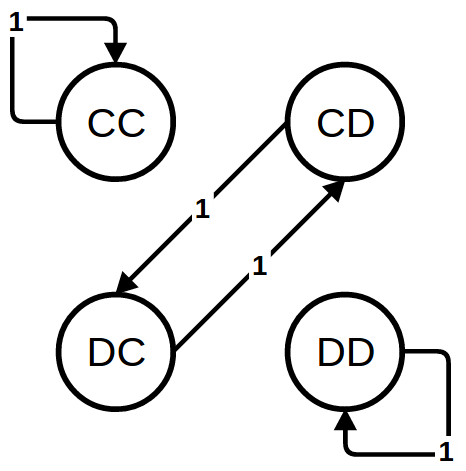
\includegraphics[width=0.28\textwidth]{state_diagram.png}
\end{center}\caption{State diagram for two TFT players} \label{fig:tft_markov}
\end{figure}
One example is \(\vec{p} = (1, 0, 1, 0)\) vs. \(\vec{q} = (1, 0, 1, 0)\), which corresponds to the state diagram shown in Figure \ref{fig:tft_markov}. The system has three steady states. First, mutual cooperation will always give rise to mutual cooperation, so if the two players start by cooperating, they will have an unbroken chain of mutual cooperation.
Second, if the two players start in the \(cd\) or \(dc\) state, then they will alternate back and forth between the states forever, and spend half their time in each state. Third and finally, the players can start in the \(dd\) state, and then remain in \(dd\) indefinitely. These correspond to the 3 left eigenvectors \((1, 0, 0, 0)\), \((0, 1, 1, 0)\), and \((0, 0, 0, 1)\) with eigenvalue 1.

The steady-states in this system feel a bit unstable. One slip, and the system will get stuck in a different loop, until another mistake is made. Another example is the case of two ``grudgers'' (who will cooperate until they are betrayed, and then never forgive their opponent) playing against each other. As soon as one makes a mistake, they will be stuck in mutual defection indefinitely. Even another mistake isn't enough to rescue the players in this case, they both need to err simultaneously to play the ``cooperate'' card in order to get back on track.

\begin{table}[h]
\centering
\resizebox{\columnwidth}{!}{%
\begin{tabular}{c r| c|c|c|c|c|c|c|c|c|c|c|c|c|c|c|c|}
\\
& \multicolumn{1}{ c }{} & \multicolumn{16}{c}{\textbf{Player 2 Strategy}} \\
& \multicolumn{1}{ c }{} &
\rot{(0, 0, 0, 0)}&
\rot{(0, 0, 0, 1)} &
\rot{(0, 0, 1, 0)} &
\rot{(0, 0, 1, 1)} &
\rot{(0, 1, 0, 0)} &
\rot{(0, 1, 0, 1)} &
\rot{(0, 1, 1, 0)} &
\rot{(0, 1, 1, 1)} &
\rot{(1, 0, 0, 0)} &
\rot{(1, 0, 0, 1)} &
\rot{(1, 0, 1, 0)} &
\rot{(1, 0, 1, 1)} &
\rot{(1, 1, 0, 0)} &
\rot{(1, 1, 0, 1)} &
\rot{(1, 1, 1, 0)} &
\rot{(1, 1, 1, 1)} \\ \cline{3-18}
\multirow{16}{*}{ \begin{sideways}\textbf{Player 1 Strategy}\end{sideways}} &(0, 0, 0, 0) &  1 & 3 & 1 & 3 & \bs & 5 & \bs & 5 & 1 & 3 & 1 & 3 & \bs & 5 & \bs & 5 \\ \cline{3-18}
&(0, 0, 0, 1) & \(1/2\) & 2 & 2 & 2 & \bs & \bs & 5 & \bs & \(1/2\) & 3 & 2 & 3 & \bs & 5 & 5 & 5 \\ \cline{3-18}
&(0, 0, 1, 0) & 1 & 2 & \bs & \(5/2\) & 1 & 3 & 1 & 3 & 1 & 2 & \bs & \(5/2\) & \bs & 4 & \bs & 4 \\ \cline{3-18}
&(0, 0, 1, 1) & \(1/2\) & 2 & \(5/2\) & \bs & \(1/2\) & 2 & \(9/4\) & 2 & \(1/2\) & \(9/4\) & \(5/2\) & \(5/2\) & \bs & 4 & 4 & 4 \\ \cline{3-18}
&(0, 1, 0, 0) & \bs & \bs & 1 & 3 & \bs & \bs & \bs & 5 & \bs & \bs & 1 & 3 & \bs & \bs & \bs & 5 \\ \cline{3-18}
&(0, 1, 0, 1) & 0 & \bs & \(4/3\) & 2 & \bs & \bs & \bs & \bs & 0 & \bs & \(9/4\) & 3 & \bs & \bs & 5 & 5 \\ \cline{3-18}
&(0, 1, 1, 0) & \bs & 0 & 1 & \(9/4\) & \bs & \bs & 1 & 3 & \bs & 0 & \bs & \(8/3\) & \bs & \bs & \bs & 4 \\ \cline{3-18}
&(0, 1, 1, 1) & 0 & \bs & \(4/3\) & 2 & 0 & \bs & \(4/3\) & 2 & 0 & 0 & \(8/3\) & \(8/3\) & \bs & \bs & 4 & 4 \\ \cline{3-18}
&(1, 0, 0, 0) & 1 & 3 & 1 & 3 & \bs & 5 & \bs & 5 & \bs & \bs & \bs & \bs & \bs & \bs & \bs & \bs \\ \cline{3-18}
&(1, 0, 0, 1) & \(1/2\) & \(4/3\) & 2 & \(9/4\) & \bs & \bs & 5 & 5 & \bs & 3 & \bs & 3 & \bs & \bs & \bs & \bs \\ \cline{3-18}
&(1, 0, 1, 0) & 1 & 2 & \bs & \(5/2\) & 1 & \(9/4\) & \bs & \(8/3\) & \bs & \bs & \bs & \bs & \bs & 3 & \bs & 3 \\ \cline{3-18}
&(1, 0, 1, 1) & \(1/2\) & \(4/3\) & \(5/2\) & \(5/2\) & \(1/2\) & \(4/3\) & \(8/3\) & \(8/3\) & \bs & 3 & \bs & \bs & \bs & 3 & 3 & 3 \\ \cline{3-18}
&(1, 1, 0, 0) & \bs & \bs & \bs & \bs & \bs & \bs & \bs & \bs & \bs & \bs & \bs & \bs & \bs & \bs & \bs & \bs \\ \cline{3-18}
&(1, 1, 0, 1) & 0 & 0 & \(3/2\) & \(3/2\) & \bs & \bs & \bs & \bs & \bs & \bs & 3 & 3 & \bs & \bs & \bs & \bs \\ \cline{3-18}
&(1, 1, 1, 0) & \bs & 0 & \bs & \(3/2\) & \bs & 0 & \bs & \(3/2\) & \bs & \bs & \bs & 3 & \bs & \bs & \bs & 3 \\ \cline{3-18}
&(1, 1, 1, 1) & 0 & 0 & \(3/2\) & \(3/2\) & 0 & 0 & \(3/2\) & \(3/2\) & \bs & \bs & 3 & 3 & \bs & \bs & 3 & 3 \\ \cline{3-18}
\end{tabular}%
} \caption{Expected scores for Player 1 calculated directly using the matrix method}\label{tab:scores_table_uncorrected}
\end{table}

How can we model this? We would like to know what the expected score for these pairs of strategies is, given that they may make a mistake now and then. So we will build in an error parameter \(\alpha\). Say \(\alpha = 0.01\), so players make a mistake one out of every 100 turns. Then we can view the TFT strategy as \((0.99, 0.01, 0.99, 0.01)\). This has the effect of connecting the state diagram, and allows us to calculate the steady state vectors using Equation (\ref{eq:scores}). This gives an expected value of \(2.25\) for both players. This is interesting, because the \(CC\) state yields 3 points for each player, bouncing between \(CD\) and \(DC\) forever gives an expected value of \(2.5\) per turn, and \(DD\) gives \(1\) point per turn. Closer inspection reveals that the lone stationary vector is \((1, 1, 1, 1)\), so the system spends equal time in each state over an infinite period, giving an expected score of \((5)(0.25) + (3)(0.25) + (1)(0.25) + (0)(0.25) = 2.25\) for each player. Perhaps more interesting is that changing \(\alpha\) doesn't seem to have any effect on this particular system, even up to \(\alpha = 1\) (always make a mistake).

Another benefit to this model is that we know the Markov chain will always converge to the steady-state vector for any initial conditions, so whether players cooperate or defect initially is irrelevant on a long enough time scale. 

In all cases, we are able to find the limit as \(\alpha \rightarrow 0\), and deduce expected values per turn for each missing pair of strategies in Table \ref{tab:scores_table_uncorrected}. I believe this to be a valid strategy because for a given pair of strategies, a lower error rate either improves, or does not affect a player's score, so we can imagine that in real-life scenarios, there will either be a selection pressure toward low error rates, or the scores will be the same as if we had taken the limit anyway. Also, this method gives the same values for scores that we already knew from Table \ref{tab:scores_table_uncorrected}. The updated scores for each pair of strategies are shown in Table \ref{tab:scores_table_corrected}.

We can verify these scores using the \texttt{2\_player\_simulation.py}\footnote{See \url{https://github.com/ashtonbaker/math-463-project/} for all code mentioned in this project.} program I mentioned previously. Figure \ref{fig:tft_tft_simulation} shows how the per-round scores for two Tit-for-Tat players changes over time. As the model predicts, this doesn't change with different initial plays. If the two TFT players (with a small but non-zero error rate) play against each other for a long time, they can expect to spend an equal amount of time in each of the four possible states, and so gain an average of 2.25 points per round played.

\begin{figure}[h]
\begin{center}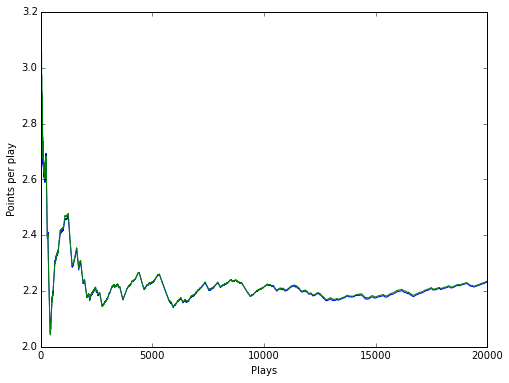
\includegraphics[width=0.48\textwidth]{tft_tft_simulation.png}
\end{center}\caption{Points-per-round for two TFT players} \label{fig:tft_tft_simulation}
\end{figure}

Now, the lower the error rate, the longer that the system spends in each type of cycle (\(cc \rightarrow cc\), \(dd \rightarrow dd\), or \(dc \rightarrow cd\)) before an error breaks the system out of the cycle. So it is conceivable that there would be a way to ``play inside'' the timescale of the Markov equilibrium. Press and Dyson show that we don't need to wait for Markov equilibrium in some cases, but it would be worth investigating the effects of changing error for each player, and the effects of shortening the timescale of the games. It is possible that for given pairs of strategies, and short time scales, a player could improve their score by playing with a different error rate, with the knowledge that the game will not reach Markov equilibrium any time soon.


\begin{table}[h]
\centering
\resizebox{\columnwidth}{!}{%
\begin{tabular}{c r| c|c|c|c|c|c|c|c|c|c|c|c|c|c|c|c|}
\\
& \multicolumn{1}{ c }{} & \multicolumn{16}{c}{\textbf{Player 2 Strategy}} \\
& \multicolumn{1}{ c }{} &
\rot{(0, 0, 0, 0)}&
\rot{(0, 0, 0, 1)} &
\rot{(0, 0, 1, 0)} &
\rot{(0, 0, 1, 1)} &
\rot{(0, 1, 0, 0)} &
\rot{(0, 1, 0, 1)} &
\rot{(0, 1, 1, 0)} &
\rot{(0, 1, 1, 1)} &
\rot{(1, 0, 0, 0)} &
\rot{(1, 0, 0, 1)} &
\rot{(1, 0, 1, 0)} &
\rot{(1, 0, 1, 1)} &
\rot{(1, 1, 0, 0)} &
\rot{(1, 1, 0, 1)} &
\rot{(1, 1, 1, 0)} &
\rot{(1, 1, 1, 1)} \\ \cline{3-18}
\multirow{16}{*}{ \begin{sideways}\textbf{Player 1 Strategy}\end{sideways}} & (0, 0, 0, 0) & 1 & 3 & 1 & 3 & \(7/3\) & 5 & 3 & 5 & 1 & 3 & 1 & 3 & 3 & 5 & \(11/3\) & 5 \\ \cline{3-18}
&(0, 0, 0, 1) & \(1/2\) & 2 & 2 & 2 & \(7/5\) & 3 & 5 & \(7/2\) & \(1/2\) & 3 & 2 & 3 & \(11/4\) & 5 & 5 & 5 \\ \cline{3-18}
&(0, 0, 1, 0) & 1 & 2 & \(7/4\) & \(5/2\) & 1 & 3 & 1 & 3 & 1 & 2 & 2 & \(5/2\) & \(5/2\) & 4 & \(17/5\) & 4 \\ \cline{3-18}
&(0, 0, 1, 1) & \(1/2\) & 2 & \(5/2\) & \(5/4\) & \(1/2\) & 2 & \(5/4\) & 2 & \(1/2\) & \(5/4\) & \(5/2\) & \(5/2\) & \(5/4\) & 4 & 4 & 4 \\ \cline{3-18}
&(0, 1, 0, 0) & \(2/3\) & \(12/5\) & 1 & 3 & \(7/4\) & 5 & \(7/3\) & 5 & \(2/3\) & \(12/5\) & 1 & 3 & \(17/6\) & 5 & \(11/3\) & 5 \\ \cline{3-18}
&(0, 1, 0, 1) & 0 & \(4/3\) & \(4/3\) & 2 & 0 & \(5/4\) & \(5/4\) & 3 & 0 & \(5/4\) & \(5/4\) & 3 & \(5/2\) & 5 & 5 & 5 \\ \cline{3-18}
&(0, 1, 1, 0) & \(1/2\) & 0 & 1 & \(5/4\) & \(2/3\) & \(5/4\) & 1 & 3 & \(1/3\) & 0 & \(5/4\) & \(8/3\) & \(5/4\) & \(16/5\) & \(17/5\) & 4 \\ \cline{3-18}
&(0, 1, 1, 1) & 0 & 1 & \(4/3\) & 2 & 0 & \(4/3\) & \(4/3\) & 2 & 0 & 0 & \(8/3\) & \(8/3\) & 2 & \(16/5\) & 4 & 4 \\ \cline{3-18}
&(1, 0, 0, 0) & 1 & 3 & 1 & 3 & \(7/3\) & 5 & \(11/3\) & 5 & 1 & 3 & 1 & 3 & \(8/3\) & \(13/3\) & \(7/2\) & \(13/3\) \\ \cline{3-18}
&(1, 0, 0, 1) & \(1/2\) & \(4/3\) & 2 & \(5/4\) & \(7/5\) & \(5/4\) & 5 & 5 & 1 & 3 & \(5/4\) & 3 & \(5/4\) & \(11/3\) & \(13/3\) & 4 \\ \cline{3-18}
&(1, 0, 1, 0) & 1 & 2 & 2 & \(5/2\) & 1 & \(5/4\) & \(5/4\) & \(8/3\) & 1 & \(5/4\) & \(5/4\) & \(8/3\) & 2 & 3 & 3 & 3 \\ \cline{3-18}
&(1, 0, 1, 1) & \(1/2\) & \(4/3\) & \(5/2\) & \(5/2\) & \(1/2\) & \(4/3\) & \(8/3\) & \(8/3\) & 1 & 3 & \(8/3\) & \(11/4\) & \(7/4\) & 3 & 3 & 3 \\ \cline{3-18}
&(1, 1, 0, 0) & \(1/2\) & \(3/2\) & \(5/4\) & \(5/4\) & \(1/6\) & \(5/2\) & \(5/4\) & \(13/4\) & 1 & \(5/4\) & 2 & 3 & \(5/4\) & \(7/2\) & \(10/3\) & 4 \\ \cline{3-18}
&(1, 1, 0, 1) & 0 & 0 & \(3/2\) & \(3/2\) & 0 & 0 & \(11/5\) & \(11/5\) & 1 & 2 & 3 & 3 & \(11/6\) & \(11/4\) & \(11/3\) & \(11/3\) \\ \cline{3-18}
&(1, 1, 1, 0) & \(1/3\) & 0 & \(7/5\) & \(3/2\) & \(1/3\) & 0 & \(7/5\) & \(3/2\) & 1 & 1 & 3 & 3 & \(5/3\) & 2 & 3 & 3 \\ \cline{3-18}
&(1, 1, 1, 1) & 0 & 0 & \(3/2\) & \(3/2\) & 0 & 0 & \(3/2\) & \(3/2\) & 1 & \(3/2\) & 3 & 3 & \(3/2\) & 2 & 3 & 3 \\ \cline{3-18}
\end{tabular}%
}\caption{Expected scores for Player 1 as both players' error approaches zero}\label{tab:scores_table_corrected}
\end{table}

\section{Modeling reproduction}

Now that we have a model for predicting scores between any two pairs of strategies, we can model reproduction without having to compute the results of individual games. Many models for reproduction have been used in the literature, many of which involve random mating, and passing on ``genes'', or statistical likelihood of survival based on individual scores. These all feel a bit arbitrary to me. The model I chose for reproduction is very simple. If we imagine that points are an analogue for resources, then we can imagine that a population's proportional representation in the next generation is equal to the portion of points which were earned by that population. That is, if in a given generation population \(X\) scores 30 points and \(Y\) scores 70 points, then \(X\) will make up 30 percent of the next generation, and \(Y\) will make up 70 percent. 

This model passes common-sense tests. If \(X\) scores no points, then players in \(X\) earned no resources at all, and their representation in the next generation will be zero. If \(X\) and \(Y\) score the same amount of resources, then then their representation in the next generation will be equal. Also, if \(X\) scores higher per individual, then \(X\)'s representation will improve in the next generation.

Let's say we have a population \(X\) which plays by strategy \(\vec{p}\), and a population \(Y\) which plays by strategy \(\vec{q}\). Then let \(x_i\) be the portion of the population which is \(X\), and let \(y_i\) be the portion of the population which is \(Y\) at generation \(i\). Also, let \(s_{xy}\) be the score that an \(X\) player can expect when playing against a \(Y\) player. We wish to model random interactions between players. If we choose a player from \(X\), then choose an opponent randomly, then we can expect the \(X\) player's score to be \( x_i s_{xx} + y_i s_{yy}\). Similarly, we can expect the \(Y\) player's score to be \(y_i s_{yy} + x_i s_{yx}\). So the expected values of the total scores amassed by the two populations are
\begin{equation}
\begin{aligned}
S_X &= x_i (x_i s_{xx} + y_i s_{xy}) = x_i^2 s_{xx} + x_i y_i s_{xy}\\
S_Y &= y_i (y_i s_{yy} + x_i s_{yx}) = y_i^2 s_{yy} + x_i y_i s_{yx}
\end{aligned}\label{eq:2_player_population_scores}
\end{equation}
The populations should be represented in the next generation in equal proportion to the scores they amassed, so we have the final equations
\begin{equation}
\begin{aligned}
x_{i + 1} &= \frac{S_X}{S_X + S_Y} = \frac{x_i^2 s_{xx} + x_i y_i s_{xy}}{x_i^2 s_{xx} + x_i y_i(s_{xy} + s{yx}) + y_i^2 s_{yy}} \\
y_{i + 1} &= \frac{S_Y}{S_X + S_Y} = \frac{y_i^2 s_{yy} + x_i y_i s_{yx}}{x_i^2 s_{xx} + x_i y_i(s_{xy} + s{yx}) + y_i^2 s_{yy}}
\end{aligned}\label{eq:2_player_populations}
\end{equation}


I wrote a Python script (\texttt{multi\_player\_dynamics.py}) to simulate this system, with strategies \(\vec{p}\) and \(\vec{q}\), and initial populations for each, and performed the following experiment. It is predicted that in a population of Tit-for-Tat players will take over in a population of Always Defect (ALLD) players, even if the initial number of TFT players is very small. The reason for this is that TFT players do just as badly against ALLD players as ALLD players do,
\begin{figure}[h]
\begin{center}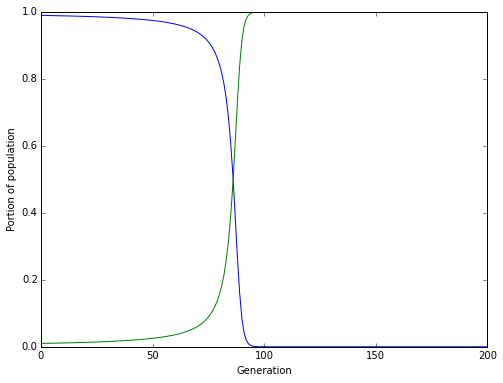
\includegraphics[width=0.48\textwidth]{2_player_dynamics.png}
\end{center}\caption{Tit-for-Tat insurgency in an Always Defect population} \label{fig:2_player_dynamics}
\end{figure}
but they have the advantage of doing well against TFT players. So they should get a higher per-player score than the ALLD population, leading to an eventual takeover. So I used my program to simulate the dynamics of this system with TFT players representing 1\% of the population initially. This gave the results shown in Figure (\ref{fig:2_player_dynamics}), which show that this prediction is correct. We would like to understand the long-term behavior of every pair of strategies in this way. I modified my program \texttt{2\_population\_simulation.py} to simulate every pair of strategies \(\vec{p}\) and \(\vec{q}\), with a small initial \(\vec{p}\), to see what happens to the populations. The results are presented here in Table \ref{tab:insurgency_outcomes}. We can see that only two strategies dominate over the Always Defect strategy. These strategies are \((0, 0, 1, 0)\) and \((1, 0, 1, 0)\). This shows that a population of defectors is not stable. Though an always-defector cannot be beaten in any individual round of the IPD, in the end cooperation between TFT players means that they amass more total points.

\begin{table}
\centering
\resizebox{\columnwidth}{!}{%
\begin{tabular}{c r| c|c|c|c|c|c|c|c|c|c|c|c|c|c|c|c|}
\\
& \multicolumn{1}{ c }{} & \multicolumn{16}{c}{\textbf{Player 2 Strategy}} \\
& \multicolumn{1}{ c }{} &
\rot{(0, 0, 0, 0)}&
\rot{(0, 0, 0, 1)} &
\rot{(0, 0, 1, 0)} &
\rot{(0, 0, 1, 1)} &
\rot{(0, 1, 0, 0)} &
\rot{(0, 1, 0, 1)} &
\rot{(0, 1, 1, 0)} &
\rot{(0, 1, 1, 1)} &
\rot{(1, 0, 0, 0)} &
\rot{(1, 0, 0, 1)} &
\rot{(1, 0, 1, 0)} &
\rot{(1, 0, 1, 1)} &
\rot{(1, 1, 0, 0)} &
\rot{(1, 1, 0, 1)} &
\rot{(1, 1, 1, 0)} &
\rot{(1, 1, 1, 1)} \\ \cline{3-18}
\multirow{16}{*}{ \begin{sideways}\textbf{Player 1 Strategy}\end{sideways}}
&(0, 0, 0, 0) & 0.01 & 1 & 0 & 1 & 1 & 1 & 1 & 1 & 0.01 & 1 & 0 & 1 & 1 & 1 & 1 & 1 \\ \cline{3-18}
&(0, 0, 0, 1) & 0 & 0.01 & 1 & 0 & 0 & 1 & 1 & 1 & 0 & 1 & 0 & 1 & 1 & 1 & 1 & 1 \\ \cline{3-18}
&(0, 0, 1, 0) & 1 & 0 & 0.01 & 0.25 & 0 & 1 & 1 & 1 & 1 & 0 & 0 & 0 & 1 & 1 & 1 & 1 \\ \cline{3-18}
&(0, 0, 1, 1) & 0 & 1 & 0.75 & 0.01 & 0 & 0 & 1 & 1 & 0 & 0 & 0.5 & 0 & 0.01 & 1 & 1 & 1 \\ \cline{3-18}
&(0, 1, 0, 0) & 0 & 1 & 0 & 1 & 0.01 & 1 & 1 & 1 & 0 & 0 & 0 & 1 & 1 & 1 & 1 & 1 \\ \cline{3-18}
&(0, 1, 0, 1) & 0 & 0 & 0 & 0 & 0 & 0.01 & 1 & 1 & 0 & 0 & 0.01 & 1 & 0.5 & 1 & 1 & 1 \\ \cline{3-18}
&(0, 1, 1, 0) & 0 & 0 & 0 & 0 & 0 & 0 & 0.01 & 0.75 & 0 & 0 & 0 & 0 & 0.00 & 0.27 & 0.5 & 0.67 \\ \cline{3-18}
&(0, 1, 1, 1) & 0 & 0 & 0 & 0 & 0 & 0 & 0.25 & 0.01 & 0 & 0 & 0.38 & 0 & 0 & 0.6 & 1 & 1 \\ \cline{3-18}
&(1, 0, 0, 0) & 0.01 & 1 & 0 & 1 & 1 & 1 & 1 & 1 & 0.01 & 0.01 & 0 & 0.1 & 1 & 1 & 1 & 0.1 \\ \cline{3-18}
&(1, 0, 0, 1) & 0 & 0 & 1 & 1 & 0 & 1 & 1 & 1 & 0.01 & 0.01 & 1 & 1 & 1 & 1 & 1 & 1 \\ \cline{3-18}
&(1, 0, 1, 0) & 1 & 1 & 1 & 0.5 & 0 & 0.01 & 1 & 0.62 & 1 & 0 & 0.01 & 0 & 0 & 0.25 & 0 & 0 \\ \cline{3-18}
&(1, 0, 1, 1) & 0 & 0 & 1 & 1 & 0 & 0 & 1 & 1 & 0 & 0 & 1 & 0.01 & 0 & 0.5 & 0 & 0 \\ \cline{3-18}
&(1, 1, 0, 0) & 0 & 0 & 0 & 0.01 & 0 & 0.5 & 1 & 1 & 0 & 0 & 0 & 1 & 0.01 & 1 & 1 & 1 \\ \cline{3-18}
&(1, 1, 0, 1) & 0 & 0 & 0 & 0 & 0 & 0 & 0.73 & 0.31 & 0 & 0 & 0.75 & 0.5 & 0 & 0.01 & 1 & 1 \\ \cline{3-18}
&(1, 1, 1, 0) & 0 & 0 & 0 & 0 & 0 & 0 & 0.5 & 0 & 0 & 0 & 1 & 1 & 0 & 0 & 0.01 & 0.01 \\ \cline{3-18}
&(1, 1, 1, 1) & 0 & 0 & 0 & 0 & 0 & 0 & 0.33 & 0 & 0 & 0 & 1 & 1 & 0 & 0 & 0.01 & 0.01 \\ \cline{3-18}
\end{tabular}%
}\caption{Eventual population for Player 1 after starting as 1\% of the population}\label{tab:insurgency_outcomes}
\end{table}

However, Table \ref{tab:insurgency_outcomes} shows that a population of TFT is not stable either! Tit-for-Tat is beaten by the overly-kind Always Cooperate strategy \((1, 1, 1, 1)\). This is because Always Cooperate spends nearly 100 percent of its time in the \(CC\) state when playing against other Always Cooperate players, so they amass even more points than the TFT population.

The table also shows that Always Cooperate is beaten by Always Defect. Always Cooperate scores no points against ALLD players, and the boost in points against other ALLC players is not enough to make up for this. This is a candidate for the ``rock-paper-scissors'' dynamics described by Axelrod, so we would like to know if this system oscillates. To do this, we must now develop a model for multi-species interactions.

\section{Multi-population dynamics}
Finally, we will develop a set of equations to model the interactions between any number of species. Say we have a population \(\vec{p}\) consisting of \(n\) strategies \(\vec{p}_1, \vec{p}_2, \ldots, \vec{p}_n\). Then let \(s(i, j)\) be the score for strategy \(i\) against strategy \(j\). Then we can model the scores of each population according to Equation (\ref{eq:2_player_population_scores}), so we have
\[S_i = p_i \sum_{j = 1}^n p_j s(i, j).\]
Then the total score amassed by every player is
\[T = \sum_{i,j = 1}^n p_i p_j s(i, j),\]
and the individual proporational scores can be modeled after Equation (\ref{eq:2_player_populations}) as
\[s_i = \frac{\sum_{i = 1}^n}{p_i p_j s(i, j)}{\sum_{i,j = 1}^n p_i p_j s(i, j)}\]
The population of strategy \(p_i\) in the subsequent population is equal to \(s_i\). Note that everything involved in this equation can be determined analyitically using the methods described before. So there is no simulation of individual games or statistical simulation of reproduction.

My program \texttt{multi\_player\_dynamics.py} incorporates these equations in order to simulate the behavior of systems with 2 or more players. I found that if the population of one species was too low (e.g. \(10^{-300}\)), the population would never rebound even if it technically should, so I forced the populations to never go below \(0.001\).

To simulate our ``rock-paper-scissors'' system, I used \(\vec{p}_1 = (0, 0, 0, 0)\), \(\vec{p}_2 = (1, 0, 1, 0)\), and \(\vec{p}_3 = (1, 1, 1, 1)\). I started each strategy as 1/3 of the total population. This gave the results shown in Figure \ref{fig:multi_player_dynamics}. We see the kind of oscillations we predicted, and the oscillations continue indefinitely. This is significant, because it shows that there might not be a strategy which is stable against all possible insurgent strategies. Of course, we have only looked at a small subset of the space of all possble strategies, so it's impossible to draw any conclusions based on this work.

\begin{figure}[h]
\begin{center}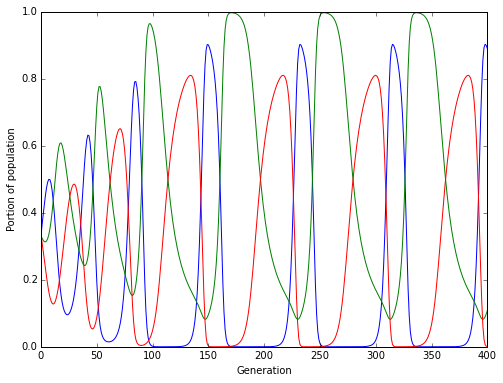
\includegraphics[width=0.48\textwidth]{multi_player_dynamics.png}
\end{center}\caption{ALLC vs ALLD vs TFT} \label{fig:multi_player_dynamics}
\end{figure}

\section{Conclusion and future work}
We have developed a model for predicting scores between any two players in a stochastic IPD game, given that the players are prone to error at a certain rate. As mentioned before, we assumed that the expected player scores could be estimated by the Markov equilibrium for the system, for any starting values. It would be worthwhile to investigate how changing the starting values changes the expected player scores. If defecting on the first move gives a higher result over the first 100 moves, then perhaps we should expect players to defect on the first move. In contrast to the Prisoner's Dilemma in general, I found this not to be the case in many situations. For example, when playing TFT vs TFT, a player cannot improve his short-term results by defecting on the first turn. I suspect this is usually the case, or at least among ``strong'' strategies such as TFT, but it would make for an interesting follow-up.

The ``rock-paper-scissors'' behavior of ALLD vs ALLC vs TFT was identified based on intutition, and using Table \ref{tab:insurgency_outcomes}. A more thorough analysis of the behavior of different groups of strategies would also be interesting to see. I don't think there's anything more complex than oscillations that can happen in this system, but it would be interesting to see which strategies converge to zero, which converge to non-zero numbers, and which oscillate. I suspect that there are systems which exhibit a ``damped'' oscillation behavior, rather than the infinite oscillations we saw in Figure \ref{fig:multi_player_dynamics}. Much more analysis could be done ton investigate this.

Finally, we only considered cases where the strategies were composed of 0's and 1's. Much of the interesting behavior in \cite{nowak_game-dynamical_1989} was obtained using other values for the strategies. Of course, there are an infinite number of such strategies, and it is difficult to characterize them all at once as we have done with the 0-and-one strategies. My assumption here was that 0-and-1 strategies give a fairly representative sample of strategies in general, and that most of the most interesting and strong strategies exist on the corners of \([0, 1]^4\). This may not be the case, but to my knowledge, no one has yet described a ``best'' strategy for the IPD.

Strategies are still being devised for the IPD. A strategy called Pavlov, which is \((1, 0, 0, 1)\) was found to be effective against TFT but not against ALLD \cite{nowak_strategy_1993}. Press and Dyson discovered so-called Zero-Determinant strategies, in which one player with a good estimate for his opponent's naive stochastic strategy may freely set his opponent's score \cite{press_iterated_2012}. Although this sounds like an unbeatably powerful strategy, it turns out that ZD strategies don't do well against themselves in populations, so they are not evolutionarily stable \cite{adami2013evolutionary}.

In reality, we can expect that new strategies are introduced to a population continually, take over, and are later killed off by some new insurgent strategy. It is possible that the natural state of this type of system is to be constantly in flux, and so there may not be a simple answer to the question of optimal animal cooperation.

\bibliography{bibliography.bib}{}
\bibliographystyle{plain}

\end{document}
